\documentclass{beamer}
\usetheme{Singapore} % Szeged, Singapore
\usepackage{etex}

% BASIC PACKAGES
% Support for Danish characters UTF-8
\usepackage{ucs}
\usepackage[utf8x]{inputenc}

%Enumerate
\usepackage{enumerate}

% English bibliography
\usepackage[english]{babel}

% Coloring of text and tables
\usepackage{color}
\usepackage{colortbl}

% Framed boxes
\usepackage{framed}

% Allow for custom floats
\usepackage{float}

% Landscape environment
%\usepackage{lscape}

% inline lists
\usepackage{paralist}

%For ensuring space after commands
\usepackage{xspace}

% Compact itemize
%\usepackage{mdwlist}

% MATHEMATICS
\usepackage{amsthm}			% AMS theorem package
\usepackage{amsfonts}
\usepackage{amsmath}		% AMS math symbols
%\usepackage{amssymb}		% More symbols!
\usepackage{mathtools}		% Even more symbols!
\usepackage{latexsym}		% Holy shit I can't believe there are still more symbols!
\usepackage{stmaryrd}		% Symbols! When will it end?
%\usepackage{textcomp}		% The unholy God of symbols has spoken. We need more symbols
%\usepackage{gensymb}
\usepackage{bussproofs}		% For making prettier type trees!

%Multiline comments etc..
\usepackage{verbatim} 

%Hopefully give us definitions..
%\input{Definitions.tex}

%Support for figures and various stuff for tables
%\usepackage[pdftex]{graphicx}	% JPEG, PNG
%\usepackage{caption}			% Put captions on everything, including stuff you can't normally do it to (for example subfigures)
\usepackage{wrapfig}			% Stuff for wrap figs
\usepackage{subfig}				% insert several subfigures in a figure
\usepackage{flafter}			% prevents floats from appearing before their definiton
\usepackage{sidecap}			% Allows text next to image
\usepackage{array}				% Used with tables - give the ability to align text to center or bottom of cell.
\usepackage{multirow}			% Used to create multi column and multi row spanning cells.
\usepackage{multicol}			% Same as multirow, but for columns. (This package may be redundant)
\usepackage{longtable}			% Tables split over several pages
\usepackage{slashbox}			% Slashed cells, eg. boxes that are split diagonally
%Path for images, images are in image/, compiled images are in bin/images/
\graphicspath{{bin/images/}}
%Allow LaTeX to accept images with dot in the filename
\usepackage{grffile}

% tikz
%\usepackage[version=0.96]{pgf}
%\usepackage{tikz}
%
\usetikzlibrary{petri,arrows,shapes,backgrounds,automata,positioning,fit}
\tikzstyle{arc}=[->,>=stealth,thick]
\tikzstyle{transportArc}=[->,>=diamond,thick]
\tikzstyle{inhibArc}=[->,>=o,thick]
\tikzstyle{every place}=[circle,thick,draw=black!75,fill=black!10,minimum size=6mm]
\tikzstyle{every transition}=[thick,draw=black,fill=black!75,minimum width=2mm,minimum height=5mm]
\tikzstyle{every token}=[fill=black,text=black]
\tikzstyle{dots}=[circle,text=black,minimum size=6mm]
\newcommand{\tzbox}[2]{\matrix(#1){#2\\}; }




\usepackage{pgfplots}
\pgfplotsset{width=5cm}

% Conditionals nice
\usepackage{ifthen}

% Really, really slack formatting
% This relaxes what is considered "bad" formatting,
% and should suppress warnings ala "underfull \hbox" and the like
\tolerance=10000            % Knuth-infinite
\hbadness=10000
\emergencystretch=1.5em     % EMERGENCY STETCH
\hfuzz 10000pt
\widowpenalty=10000
\vfuzz \hfuzz
\raggedbottom

%See http://www.eng.cam.ac.uk/help/tpl/textprocessing/squeeze.html
\setlength{\intextsep}{1.5ex}

% Different font in captions
\newcommand{\captionfonts}{\small}

\makeatletter  % Allow the use of @ in command names
\long\def\@makecaption#1#2{%
  \vskip\abovecaptionskip
  \sbox\@tempboxa{{\captionfonts #1: #2}}%
  \ifdim \wd\@tempboxa >\hsize
    {\captionfonts #1: #2\par}
  \else
    \hbox to\hsize{\hfil\box\@tempboxa\hfil}%
  \fi
  \vskip\belowcaptionskip}
\makeatother   % Cancel the effect of \makeatletter

% ALGORITHMS%
%\usepackage{algorithmic}
\usepackage[ruled]{algorithm}
\usepackage{algpseudocode}
%Algorithmic should use "Input:" and "Output:" instead of "require:" and "ensure:"
\algrenewcommand{\algorithmicrequire}{\textbf{Input:}}
\algrenewcommand{\algorithmicensure}{\textbf{Output:}}

% CUSTOM MACROS
\newcommand{\tech}{SFRAVTLS\xspace}

% METADATA
\author{Karsten Jakobsen and Sabrine Mouritsen}
\title{Simulating Fuel Reduction by Adjusting Velocity to Traffic Lights}
\pagenumbering{arabic}

\setbeamertemplate{footline}[page number]


\begin{document}
\begin{frame}[plain]
  \titlepage
\end{frame}

\AtBeginSection[]{
	\frame<beamer>{ 
		\frametitle{Table of Contents}   
		\tableofcontents[currentsection,subsections] 
 	}
}

\begin{frame}{Table of Contents}
\pdfbookmark[0]{Contents}{toc}
\setcounter{tocdepth}{1}
\tableofcontents
\setcounter{tocdepth}{2}
\end{frame}


%%%%%%%%%% DO NOT EDIT BELOW, THIS WILL BE AUTO GENERATED %%%%%%%%%%
% Model - med figur
% Algorithm - som figur
% Animationer
% Demo af sumo

\section{Solution}
\subsection{Model}
\begin{frame}{Model}
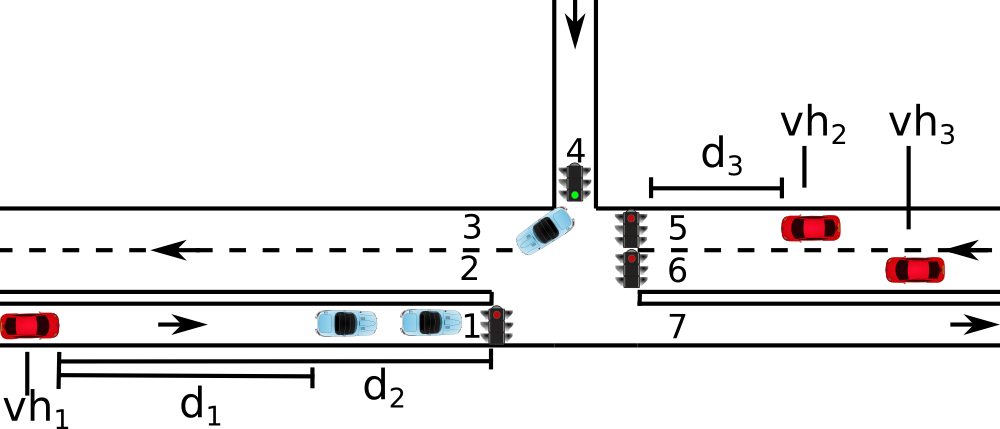
\includegraphics[width=1\textwidth]{images/introNetwork.png}
\end{frame}

\begin{frame}{Space Model}
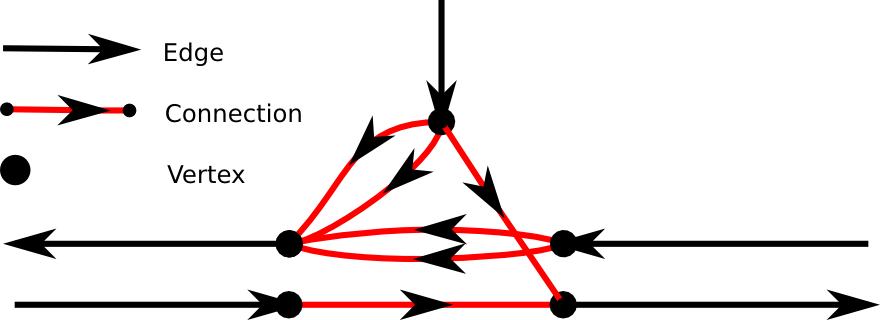
\includegraphics[width=1\textwidth]{images/ConnectionNetwork.png}
\end{frame}

\subsection{Algorithm}
\begin{frame}{Algorithm}
\begin{itemize}
\item In a junction
\item Calculate distance
\item Phase conversion
\item Calculate velocity
\end{itemize}
\end{frame}
\begin{frame}{In Junction}
\begin{center}
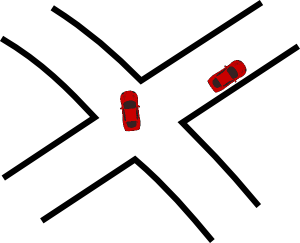
\includegraphics[width=0.8\textwidth]{images/algjuction.png}
\end{center}
\end{frame}

\begin{frame}{Calculate Distance}
\begin{center}
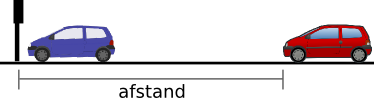
\includegraphics[width=1\textwidth]{images/algdistance.png}
\end{center}
\end{frame}

\begin{frame}{Phase Conversion}
\begin{columns}
	\begin{column}{0.3\textwidth}
	\begin{center}
	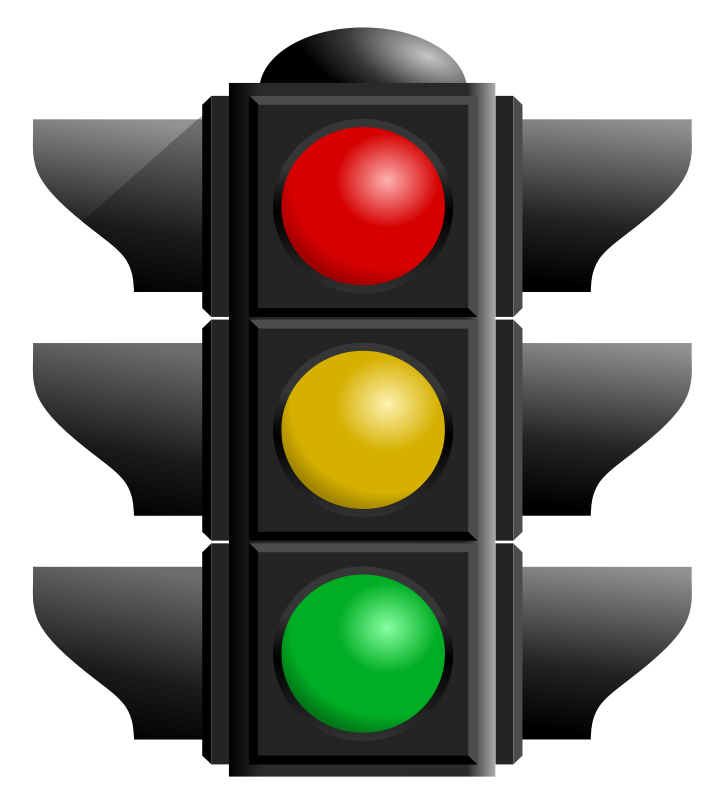
\includegraphics[width=1\textwidth]{images/traffic_light.png}
	\end{center}
	\end{column}

	\begin{column}{0.4\textwidth}
	\begin{center}
	\begin{tabular}{lll}
	\multicolumn{3}{l}{\textbf{Phase:}} \\
	green & : & 30 s \\
	yellow & : &  4 s \\
	red & : & 15 s \\
	yellow & : & 2 s \\
	green & : & 30 s\\
	\ \ \ \vdots&&\\
	\end{tabular}
	\end{center}
	\end{column}

	\begin{column}{0.3\textwidth}
	\begin{center}
	\begin{tabular}{l}
	\textbf{Green spans:} \\
	now: 42 s\\
	(51, 81) \\
	(102, 132) \\
	(153, 183) \\
	\ \ \ \ \vdots\\\\
	\end{tabular}
	\end{center}
	\end{column}
\end{columns}
\end{frame}

\begin{frame}{Calculate Velocity}
\[velocity = \frac{distance}{time}\]
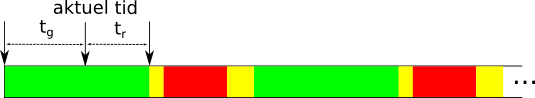
\includegraphics[width=1\textwidth]{images/algphases1.png}
\end{frame}

\begin{frame}{Calculate Velocity}
\[velocity = \frac{distance}{time}\]
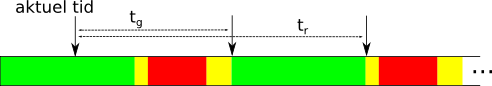
\includegraphics[width=1\textwidth]{images/algphases2.png}
\end{frame}

\begin{frame}{Calculate Velocity}
\[velocity = \frac{distance}{time}\]
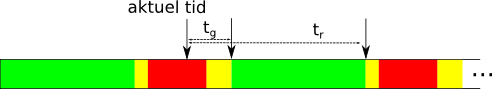
\includegraphics[width=1\textwidth]{images/algphases3.png}
\end{frame}







%%%%%%%%%% DO NOT EDIT ABOVE, THIS WILL BE AUTO GENERATED %%%%%%%%%%

\end{document}